\chapter{Neural Network Detectors}
\todo{bla}
NNs vs ML
define (NNs) abbr.

\section{Precision Metrics}
mAP, IoU

\section{Classification networks}
\label{chapt:cnets}
In order to better understand detection networks, we will shortly describe their predecessors, classification networks. Classification network is a convolutional neural network (CNN) \cite[ch.~9]{bib:dlbook} that given an image, returns a confidence score of correspondence to each of the classes. Usually, \textit{soft-max} function is applied to the confidence score to represent a probability distribution. The \textit{ImageNet} image recognition challenge\footnote{\url{http://www.image-net.org/challenges/LSVRC/}} is usually used to benchmark the accuracy of such networks.

Later, in \cref{chapt:models}, we will see how a classification model can be used as a backbone for a detector network.

\subsection*{AlexNet (2012)}
A significant breakthrough in use of CNNs happened in 2012, when the \textit{AlexNet} \cite{bib:alexnet} won the \textit{ImageNet} image recognition challenge. It was the first time a deep CNN performed better than traditional computer vision and machine learning approaches. 

AlexNet has a simple architecture with five convolutional layers and two fully connected layers, followed by a softmax layer. It has created a foundation on which today's state-of-the-art models are built and set a new standard for image recognition.

\subsection*{VGG (2014)}
\label{sec:VGG}
The network architecture, mostly known as VGG \cite{bib:vgg}, pushed the concept of AlexNet even further and has proved the feasibility of deep network with small convolutions. 

Each of the VGG's convolutional filters uses 3$\times$3 kernel and the depth of the filters is increased through the network, reaching 512 filters in the last layers. Three fully connected layers and softmax are applied after the convolutions, see \cref{tab:vggarch}. There are multiple versions of the VGG architecture, depending on the number of convolutional layers, the most popular is the 16 layer version. 

VGG network is considered a general architecture for a classification network due to its linear architecture with decreasing size of the features and increasing number of channels. 

\begin{table}[]
    \centering
    \rotatebox{90}{
        \vggArch
    }
    \caption{Architecture of VGG network, version D. Taken from \cite[table 1]{bib:vgg}}
    \label{tab:vggarch}
\end{table}
    
\subsection*{Inception (v1) (2014)}
\label{sec:inception}
Previous architectures showed that increasing the number of layers and layer size, leads to better precision. Inception v1 \cite{bib:googlenet}, also known as GoogLeNet, aims at increasing precision while improving utilization of computing resources.

In order to avoid the growing cost of stacking more layers, the network introduces the concept of sparsity by using the \textit{inception modules}, \cref{fig:incept_mod}. A sparse structure is approximated by using multiple convolutions with different kernel sizes and concatenating the outputs together. Max-pooling is also performed as an alternative to convolutions and concatenated to the output. Because high dimensional convolutions are costly, a reduction to the channels is introduced by using 1$\times$1 convolution as a preceding layer.

The network is then formed by linearly stacking nine inception modules, preceded by a linear stem network and followed by a fully connected classifier. Two auxiliary classifiers are added to intermediate layers of the network to help propagate gradients and provide regularization during the training.

A set of improvements to the Inception network was introduced in later versions of the network. Most notably a factorization of convolution layers was introduced in Inception v2 and v3 \cite{bib:inception2}.


\begin{figure}
    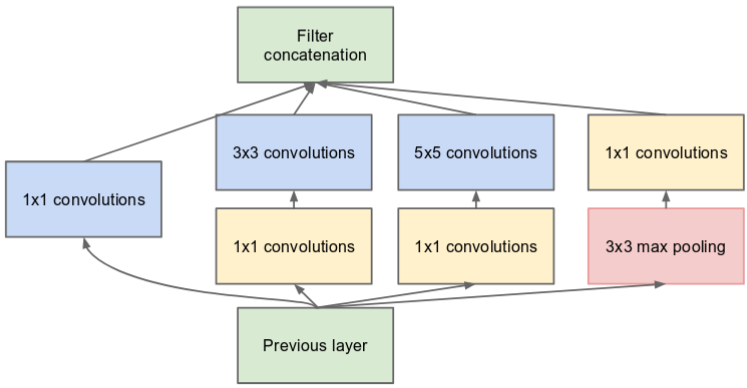
\includegraphics[width=\textwidth]{img/inception}
    \caption{Inception module, picture from \cite[figure 2]{bib:googlenet}.}
    \label{fig:incept_mod}
\end{figure}

\subsection*{ResNet (2015)}
\label{sec:resnet}

Although it has become possible to train deeper and deeper CNNs, degradation has eventually been observed. Adding more layers to models started to produce higher training error. Theoretically, adding more layers to a smaller model should produce at least equal results, as the smaller model is the subspace of the larger one. A solution to this problem was proposed in the ResNet architecture, by directly introducing identity functions to the network \cite{bib:resnet}.  

A baseline of ResNet is directly inspired by VGG (\cref{sec:VGG}). Most of the convolutional layers have 3$\times$3 filters and follow two simple rules: keep the number of filters the same, unless changing the output size and double the filters if the feature size if halved. A residual connection is then added to each pair of the convolutional layers, this connection is either an identity or a projection done by 1$\times$1 convolution to match the increased number of filters. 

\begin{figure}
    \resnetArch
    \caption{Architecture of the ResNet network and residual blocks. Each of the four \textit{Layers} are created by stacking multiple residual blocks.}
    \label{fig:resnet_arch}
\end{figure}

We can see the high level architecture of this model in \cref{fig:resnet_arch} (left). Each of four \textit{Layers} is composed of multiple linearly stacked residual blocks, exact numbers of blocks can be found in \cite[table 1]{bib:resnet}. A feature map size is preserved inside each of the \textit{Layers} and halved between them. A type of residual block we described previously was a \textit{Basic block} with two convolutional layers and is used for smaller ResNet models (ResNet-18, ResNet-34). Deeper ResNet models (ResNet-50, ResNet-101, ResNet-152) use the \textit{Bottleneck block} with three convolutional layers, where the 1$\times$1 layers are responsible for reducing and then restoring dimensions, leaving the 3$\times$3 layer a with smaller input and output dimensions. Remarkably, the 152-layer ResNet has lower complexity than the 16-layer VGG network.



\subsection*{Xception (2017)}
\label{sec:xception}

\subsection*{NasNet (2017)}
\label{sec:nasnet}

\subsection*{Present day networks}
 comparing \cref{fig:cnncomp}

\begin{figure}
    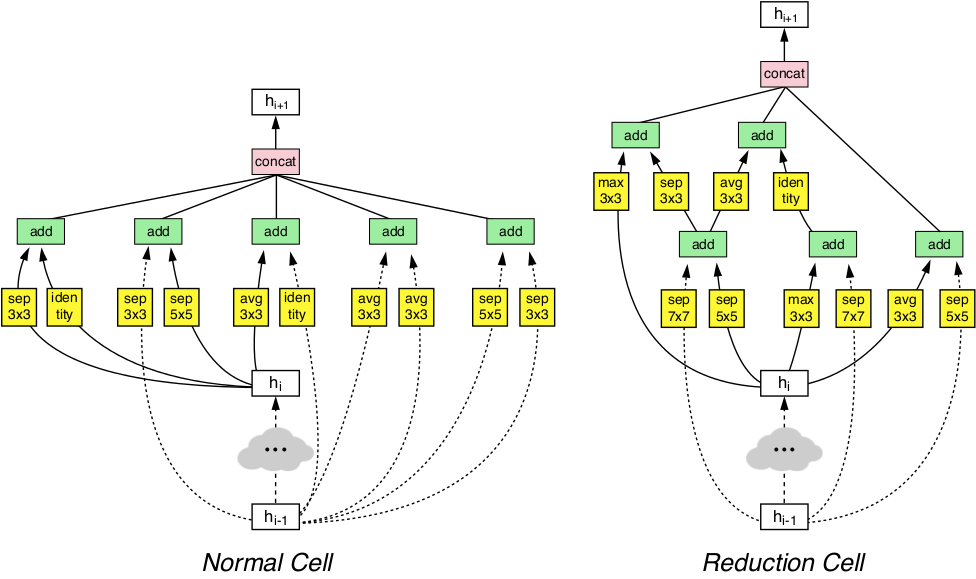
\includegraphics[width=\textwidth]{img/nasnet}
    \caption{Accuracy versus computational demand across top performing published CNN architectures on ImageNet 2012 ILSVRC challenge prediction task. Computational demand is measured in the number of floating-point multiply-add operations to process a single image. Taken from \cite{bib:nasnet}.}
    \label{fig:cnncomp}
\end{figure}

\todo{add comp table for all models}

\section{Detection networks}
\label{chapt:models}

\todo{bla}

\subsection*{Region-based Convolutional Network (R-CNN)}
\subsubsection{R-CNN}
\subsubsection{Fast R-CNN}
\subsubsection{Faster R-CNN}

\subsection*{Mask Region-based Convolutional Network (Mask R-CNN)}

\subsection*{You Only Look Once (YOLO)}
\subsubsection{YOLO}
\label{sec:yolo}
\subsubsection{YOLO v2 and YOLO 9000}

\subsection*{Single-Shot Detector (SSD)}
\label{sec:ssd}
\subsubsection{SSD}

\subsubsection{FSSD}
\subsubsection{RFB}


\section{Use of Detection networks for video processing}

%Optional section
% \section{Other uses of CNNs}
% \subsection{Noise removal/ Regularization}
% \subsection{Image generation}





